\section{Problem}

Designing and implementing a programming language and its supporting tools (collectively, a \emph{programming system}) that simultaneously supports a natural programming style, helps users find and fix errors early, and performs well across diverse problem domains remains a grand challenge in computing. Indeed, it is now widely acknowledged that no simple set of constructs will be able to handle all of the challenges modern computing faces. Consistent with this view, a large number of researchers and domain experts in both research and industry are actively engaged in the design, implementation and analysis of a variety of novel language-based abstractions, compilation strategies and tools targeted at different problem domains.

%In implementing a new feature or abstraction, these experts can take one of several approaches. 
To realize a new feature or abstraction, these experts often take a \emph{language-oriented approach}, whereby the new constructs are developed and distributed together with a new programming language. The flexibility of this approach, coupled with support from tools like compiler generators, has led to a proliferation of specialized languages, each built around a particular set of privileged constructs. Unfortunately, a key issue limiting the practicality of this approach occurs at the boundaries between languages -- specialized constructs particular to one language cannot always be safely and naturally expressed in another, so building a program out of components written in different specialized languages can often prove difficult. 

One common strategy that partially addresses this problem is to target an established language and runtime, such as the Java Virtual Machine (JVM), and support a superset of its features. This only solves the interoperability problem in one direction. While calling from the new language to the old language becomes straightforward, calls in the other direction, or between languages sharing a common target, remain restricted by the constructs available in the common language. This issue is illustrated in Figure \ref{approaches}a. This restriction can  constrain the design of new languages to only include constructs that can be expressed reasonably naturally in the target language. More novel innovations are often difficult to translate into familiar forms, however. For instance, the module system in F\# is severely constrained relative to the module system in its predecessor, OCaml, due to the need for interoperability with other CLI languages.

Stepping back, it is clear that a \emph{library-oriented approach}, shown in Figure \ref{approaches}b, where new constructs are implemented entirely within a single host language as libraries, should be preferred when possible.
% -- library-based constructs cannot interfere with one another (assuming a suitable namespacing standard), libraries benefit from common distribution infrastructure and tool support, and externally-accessible library interfaces need not be restricted to a fixed common subset of all available constructs (e.g. the object system of the JVM or CLI).  We diagram this key latter distinction in Figure \ref{approaches}. 
Of course, this is very often \emph{not} possible today because from the perspective of a library developer, the programming system is a largely inflexible, \emph{monolithic} entity. That is, the language's syntax, type checking rules and semantics are fixed in advance, the compiler is a black box implementation of these rules, and the tools operate according to domain-agnostic protocols that use only the declared structure of the program being developed as input. To enhance any of these aspects of the programming system, the expert must step out of the language, and often out of the programming system entirely. 

To put it another way, monolithic programming languages enforce a fundamental dichotomy between \emph{first-class constructs}, which enjoy support throughout the programming system but must be designed and implemented by the system designer in advance, and \emph{user-defined constructs}, which can be distributed as user libraries, but must creatively combine and repurpose the small set of available first-class constructs to express all desired run-time, compile-time and edit-time behaviors. This dichotomy has forced researchers and domain experts who want to significantly advance the state-of-the-art in programming systems, particularly in compiled, statically-typed systems where this dichotomy is most salient, to design a new language in many cases. But this then couples their core innovations with a collection of other, unrelated design choices, requires more effort both for the experts developing the innovation and its targetted user community, and leads to the intrinsic interoperability problems described above for users developing applications consisting of components written in different languages.

\begin{figure}
\begin{center}
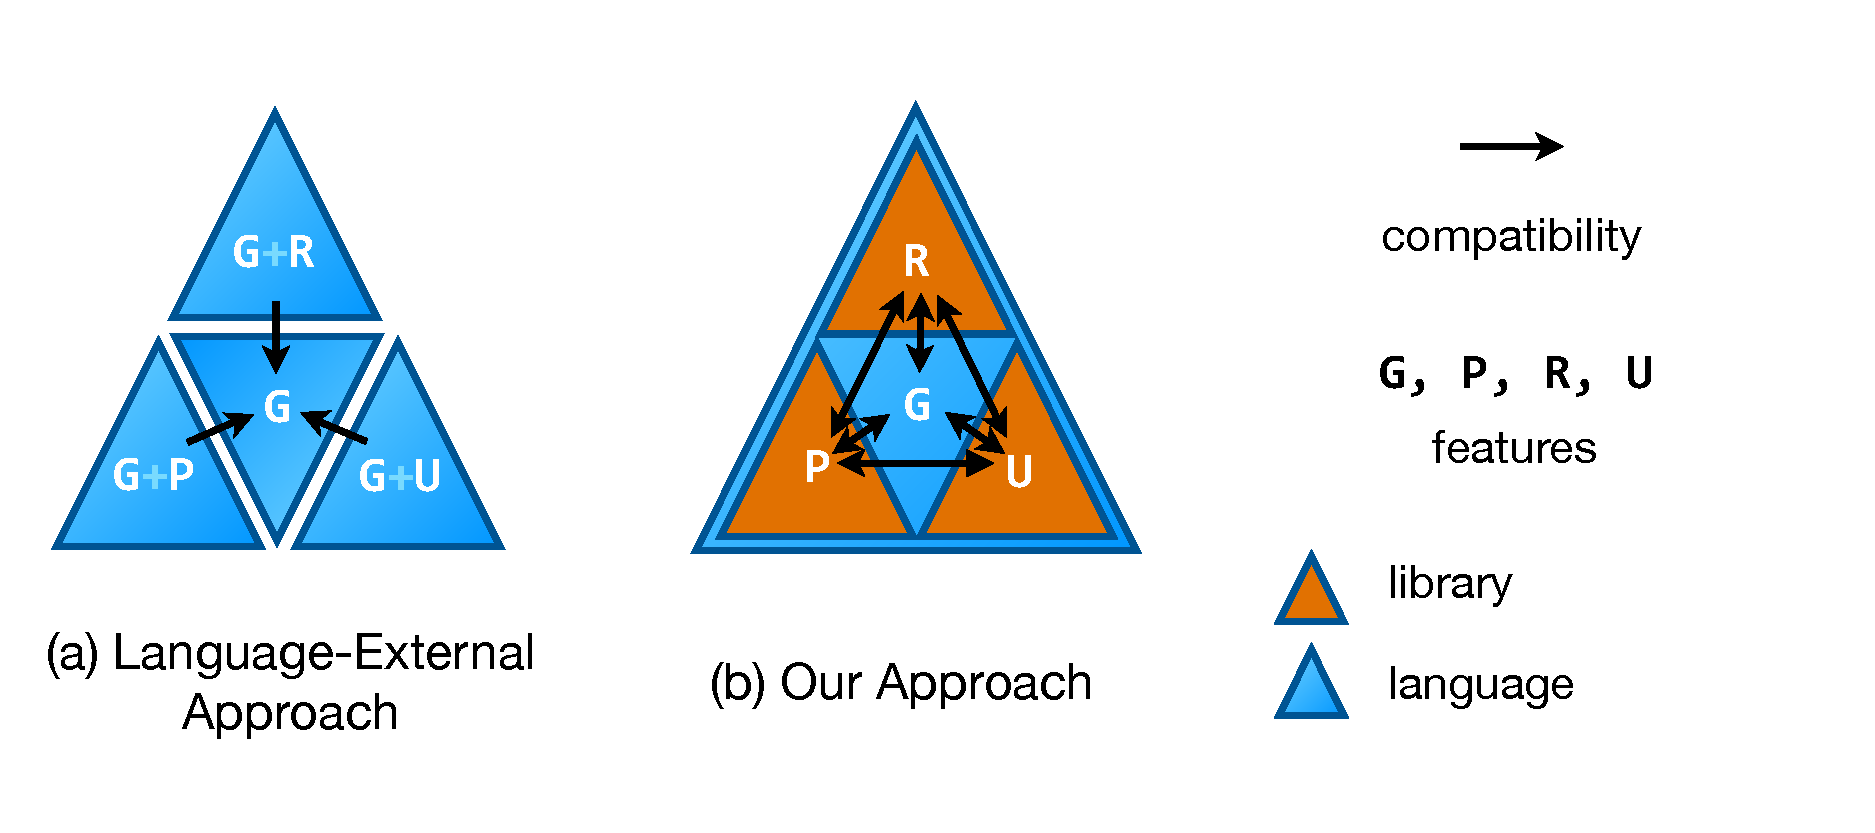
\includegraphics[scale=0.5]{approaches.pdf}
\end{center}
\vspace{-20px}
\caption{\small (a) With the language-oriented approach, novel constructs are packaged into separate languages. Users can only safely and naturally call into languages consisting of common constructs. (b) With the library-oriented approach, there is one language and novel constructs are packaged as normal libraries. Thus, interoperability is not a problem but in monolithic systems, this approach is less expressive.\label{approaches}}
\end{figure}